\documentclass[xetex,mathserif,serif]{beamer}
\usepackage{polyglossia}
\setdefaultlanguage[babelshorthands=true]{russian}
\usepackage{minted}
\usepackage{tabu}
\usepackage{moresize}

\useoutertheme{infolines}

\usepackage{fontspec}
\setmainfont{FreeSans}
\newfontfamily{\russianfonttt}{FreeSans}

\definecolor{links}{HTML}{2A1B81}
\hypersetup{colorlinks,linkcolor=,urlcolor=links}

\tabulinesep=1.2mm

\title{Ликбез по F\#}
\author{Юрий Литвинов}
\date{14.07.2021г}

\begin{document}

    \frame{\titlepage}

    \section{Введение}

    \begin{frame}
        \frametitle{Функциональное программирование}
        Программа как вычисление значения \textbf{выражения} в математическом смысле на некоторых входных данных.
        $$\sigma' = f(\sigma)$$
    
        \begin{itemize}
            \item Нет состояния $\Rightarrow$ нет переменных
            \item Нет переменных $\Rightarrow$ нет циклов
            \item Нет явной спецификации потока управления
        \end{itemize}
        Порядок вычислений не важен, потому что нет состояния, результат вычисления зависит только от входных данных.
    \end{frame}
    
    \begin{frame}[fragile]
        \frametitle{Сравним}
        \begin{alertblock}{C++}
            \begin{minted}{cpp}
int factorial(int n) {
    int result = 1;
    for (int i = 1; i <= n; ++i) {
        result *= i;
    }
    return result;
}
            \end{minted}
        \end{alertblock}
        \begin{exampleblock}{F\#}
            \begin{minted}{fsharp}
let rec factorial x =
    if x = 1 then 1 else x * factorial (x - 1)
            \end{minted}
        \end{exampleblock}
    \end{frame}

    \begin{frame}[fragile]
        \frametitle{Как с этим жить}
        \begin{itemize}
            \item Состояние и переменные <<эмулируются>> параметрами функций
            \item Циклы <<эмулируются>> рекурсией
            \item Последовательность вычислений --- рекурсия + параметры
        \end{itemize}
        \begin{exampleblock}{F\#}
            \begin{minted}{fsharp}
let rec sumFirst3 ls acc i =
    if i = 3 then 
         acc 
    else 
        sumFirst3 
            (List.tail ls) 
            (acc + ls.Head) 
            (i + 1)
            \end{minted}
        \end{exampleblock}
    \end{frame}

    \begin{frame}[fragile]
        \frametitle{Пример: функции высших порядков}
        \begin{minted}{fsharp}
let rec sumFirst3 ls acc i =
    if i = 3 then acc 
    else sumFirst3 (List.tail ls) (acc + ls.Head) (i + 1)
        \end{minted}
        $$\Downarrow$$
        \begin{minted}{fsharp}
let sumFirst3 ls = 
    Seq.fold (fun x acc -> acc + x) 0 (Seq.take 3 ls)
        \end{minted}
        $$\Downarrow$$
        \begin{minted}{fsharp}
let sumFirst3 ls = ls |> Seq.take 3 |> Seq.fold (+) 0
        \end{minted}
        $$\Downarrow$$
        \begin{minted}{fsharp}
let sumFirst3 = Seq.take 3 >> Seq.sum
        \end{minted}
    \end{frame}

    \begin{frame}[fragile]
        \frametitle{Ещё пример}
        \framesubtitle{Возвести в квадрат и сложить все чётные числа в списке}
        \begin{minted}{fsharp}
let calculate = 
    Seq.filter (fun x -> x % 2 = 0) 
    >> Seq.map (fun x -> x * x) 
    >> Seq.reduce (+)
        \end{minted}
    \end{frame}

    \section{F\#}

    \begin{frame}
        \frametitle{F\#}
        \begin{itemize}
            \item Типизированный функциональный язык для платформы .NET
            \item НЕ чисто функциональный (можно императивный стиль и ООП)
            \item Первый раз представлен публике в 2005 г., актуальная версия --- 5.0 (10 ноября 2020 года)
            \item Создавался под влиянием OCaml (практически диалект OCaml под .NET)
            \item Использует .NET CLI
            \item Компилируемый и интерпретируемый
            \item Иногда используется в промышленности, в отличие от многих чисто функциональных языков
        \end{itemize}
    \end{frame}

    \begin{frame}
        \frametitle{Что скачать и поставить}
        \begin{itemize}
            \item Под Windows --- Visual Studio, Rider
            \item Под Linux --- Rider, Visual Studio Code + Ionide
            \item Прямо в браузере: \url{https://dotnetfiddle.net/}
        \end{itemize}
    \end{frame}
    
    \begin{frame}[fragile]
        \frametitle{Пример программы}
        \begin{minted}{fsharp}
printfn "%s" "Hello, world!"
        \end{minted}
    \end{frame}

    \section{Let-определения}

    \begin{frame}[fragile]
        \frametitle{let-определение}
        \begin{minted}{fsharp}
let x = 1
let x = 2
printfn "%d" x
        \end{minted}
        можно читать как
        \begin{minted}{fsharp}
let x = 1 in let x = 2 in printfn "%d" x
        \end{minted}
        и понимать как подстановку того, что справа от $=$ вместо того, что слева, в выражение после in
    \end{frame}

    \begin{frame}[fragile]
        \frametitle{let-определение, функции}
        \begin{minted}{fsharp}
let powerOfFour x = 
    let xSquared = x * x
    xSquared * xSquared
        \end{minted}
        \begin{itemize}
            \item Позиционный синтаксис
            \begin{itemize}
                \item Отступы строго пробелами
                \item Не надо ";"
            \end{itemize}
            \item Нет особых синтаксических различий между переменной и функцией
            \item Не надо писать типы
            \item Не надо писать \textit{return}
            \item Нет возможности вернуться из функции раньше её конца
        \end{itemize}
    \end{frame}

    \begin{frame}[fragile]
        \frametitle{Вложенные let-определения}
        \begin{minted}{fsharp}
let powerOfFourPlusTwoTimesSix n =
    let n3 =
        let n1 = n * n
        let n2 = n1 * n1
        n2 + 2
    let n4 = n3 * 6
    n4
        \end{minted}
        \begin{itemize}
            \item \textit{n3} --- не функция!
            \item Компилятор отличает значения и функции по наличию аргументов
            \item Значение вычисляется, когда до \textit{let} <<доходит управление>>, 
                    функция --- когда её вызовут. Хотя, конечно, функция --- тоже значение.
        \end{itemize}
    \end{frame}

    \section{Типы}

    \begin{frame}[fragile]
        \frametitle{Типы}
        \begin{minted}{fsharp}
let rec f x =
    if x = 1 then 
        1 
    else 
        x * f (x - 1)
        \end{minted}

        \begin{alertblock}{F\# Interactive}
            \begin{minted}{fsharp}
val f : x:int -> int
            \end{minted}
        \end{alertblock}
        Каждое значение имеет тип, известный во время компиляции
    \end{frame}

    \begin{frame}
        \frametitle{Элементарные типы}
        \begin{itemize}
            \item \textit{int}
            \item \textit{double}
            \item \textit{bool}
            \item \textit{string}
            \item ... (.NET)
            \item \textit{unit} --- тип из одного значения, (). Аналог void.
        \end{itemize}
    \end{frame}
    
    \begin{frame}[fragile]
        \frametitle{Кортежи (tuples)}
        \begin{minted}{fsharp}
let site1 = ("scholar.google.com", 10)
let site2 = ("citeseerx.ist.psu.edu", 5)
let site3 = ("scopus.com", 4)
let sites = (site1, site2, site3)

let url, relevance = site1
let site1, site2, site3 = sites
        \end{minted}
    \end{frame}

    \begin{frame}[fragile]
        \frametitle{Лямбды}
        \begin{minted}{fsharp}
let primes = [2; 3; 5; 7]
let primeCubes = List.map (fun n -> n * n * n) primes
        \end{minted}
        \begin{alertblock}{F\# Interactive}
            \begin{minted}{fsharp}
> primeCubes;;
val it : int list = [8; 27; 125; 343]
            \end{minted}
        \end{alertblock}
        \begin{minted}{fsharp}
let f = fun x -> x * x
let n = f 4
        \end{minted}
    \end{frame}

    \begin{frame}
        \frametitle{Списки}
        \begin{small}
            \begin{tabu} {| X[0.9 l p] | X[1 l p] | X[1 l p] |}
                \tabucline-
                Синтаксис                               & Описание                  & Пример                                      \\
                \tabucline-
                \everyrow{\tabucline-}
                $[]$                                    & Пустой список             & $[]$                                        \\
                $[expr; ...; expr]$                     & Список с элементами       & $[1; 2; 3]$                                 \\
                $expr :: list$                          & cons, добавление в голову & $1 :: [2; 3]$                               \\
                $[expr\ ..\ expr]$                      & Промежуток целых чисел    & $[1 .. 10]$                                 \\
                $[for\ x\ in\ list\ \rightarrow\ expr]$ & Генерированный список     & $[for\ x\ in\ 1..99\ \rightarrow\ x\ *\ x]$ \\
                $list\ @\ list$                         & Конкатенация              & $[1; 2]\ @\ [3; 4]$                         \\
            \end{tabu}
        \end{small}
    \end{frame}

    \begin{frame}[fragile]
        \frametitle{Примеры работы со списками}
        \begin{minted}{fsharp}
let oddPrimes = [3; 5; 7; 11]
let morePrimes = [13; 17]
let primes = 2 :: (oddPrimes @ morePrimes)
        \end{minted}
        \begin{minted}{fsharp}
let printFirst primes =
    match primes with
    | h :: t -> printfn "First prime in the list is %d" h
    | [] -> printfn "No primes found in the list"
        \end{minted}
    \end{frame}

    \begin{frame}[fragile]
        \frametitle{Устройство списков}
        \begin{center}
            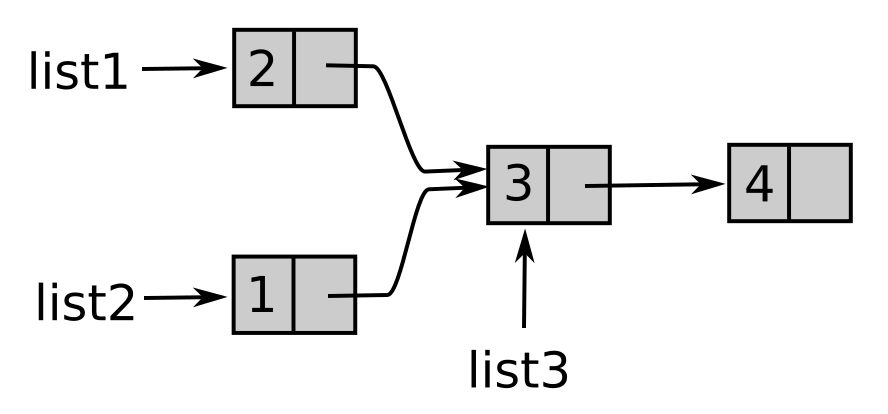
\includegraphics[width=0.4\textwidth]{lists.png}
        \end{center}
        \begin{minted}{fsharp}
let list3 = [3; 4]
let list1 = 2 :: list3
let list2 = 1 :: list3
        \end{minted}
        \begin{itemize}
            \item Списки немутабельны
            \item Cons-ячейки, указывающие друг на друга
            \item cons за константное время, @ --- за линейное
        \end{itemize}
    \end{frame}

    \begin{frame}
        \frametitle{Операции над списками}
        \framesubtitle{Модуль Microsoft.FSharp.Collections.List}
        \begin{small}
            \begin{tabu} {| X[0.5 l p] | X[1 l p] | X[1 l p] | X[0.5 l p] |}
                \tabucline-
                Функция                & Описание                            & Пример                                              & Результат            \\
                \tabucline-
                \everyrow{\tabucline-}
                List.length            & Длина списка                        & $List.length\ [1;2;3]$                              & $3$                  \\
                List.nth               & n-ый элемент списка                 & $List.nth\ [1; 2; 3]\ 1$                            & $2$                  \\
                List.init              & Генерирует список                   & $List.init\ 3 (fun\ i\ \rightarrow\ i * i)$         & $[0; 1; 4]$          \\
                List.head              & Голова списка                       & $List.head\ [1; 2; 3]$                              & $1$                  \\
                List.tail              & Хвост списка                        & $List.tail\ [1; 2; 3]$                              & $[2; 3]$             \\
                List.map               & Применяет функцию ко всем элементам & $List.map\ (fun\ i\ \rightarrow\ i * i)\ [1; 2; 3]$ & $[1; 4; 9]$          \\
                List.filter            & Отбирает нужные элементы            & $List.filter\ (fun\ x\ \rightarrow\ x\ \%\ 2 <> 0)\ [1; 2; 3]$ & $[1; 3]$  \\
                List.fold              & "Свёртка"  & $List.fold\ (fun\ x\ acc\ \rightarrow\ acc * x)\ 1\ [1; 2; 3]$               & $6$                  \\
            \end{tabu}
        \end{small}
    \end{frame}

    \begin{frame}[fragile]
        \frametitle{Тип Option}
        Либо \textit{Some что-то}, либо \textit{None}, представляет возможное отсутствие значения.
        \begin{minted}{fsharp}
let people = [ ("Adam", None); ("Eve" , None);
    ("Cain", Some("Adam","Eve"));
    ("Abel", Some("Adam","Eve")) ]
        \end{minted}
        \begin{minted}{fsharp}
let showParents (name, parents) =
    match parents with
    | Some(dad, mum) -> 
        printfn "%s, father %s, mother %s" name dad mum
    | None -> printfn "%s has no parents!" name
        \end{minted}
    \end{frame}

    \section{Функции}

    \begin{frame}[fragile]
        \frametitle{Рекурсия}
        \begin{minted}{fsharp}
let rec length l =
    match l with
    | [] -> 0
    | h :: t -> 1 + length t

let rec even n = (n = 0u) || odd(n - 1u)
and odd n = (n <> 0u) && even(n - 1u)
        \end{minted}
    \end{frame}

    \begin{frame}[fragile]
        \frametitle{Каррирование, частичное применение}
        \begin{minted}{fsharp}
let shift (dx, dy) (px, py) = (px + dx, py + dy)
let shiftRight = shift (1, 0)
let shiftUp = shift (0, 1)
let shiftLeft = shift (-1, 0)
let shiftDown = shift (0, -1)
        \end{minted}
        \begin{alertblock}{F\# Interactive}
            \begin{minted}{fsharp}
> shiftDown (1, 1);;
val it : int * int = (1, 0)
            \end{minted}
        \end{alertblock}
    \end{frame}

    \begin{frame}[fragile]
        \frametitle{Зачем --- функции высших порядков}
        \begin{minted}{fsharp}
let lists = [[1; 2]; [1]; [1; 2; 3]; [1; 2]; [1]]
let lengths = List.map List.length lists
        \end{minted}
        или
        \begin{minted}{fsharp}
let lists = [[1; 2]; [1]; [1; 2; 3]; [1; 2]; [1]]
let squares = List.map (List.map (fun x -> x * x)) lists
        \end{minted}
        \vspace{3mm}
        Функции стандартной библиотеки стараются принимать список последним, для каррирования
    \end{frame}

    \section{Композиция}

    \begin{frame}[fragile]
        \frametitle{Оператор $|>$}
        \framesubtitle{Pipe forward}
        \begin{minted}{fsharp}
let (|>) x f = f x
        \end{minted}

        \begin{minted}{fsharp}
let sumFirst3 ls = ls |> Seq.take 3 |> Seq.fold (+) 0
        \end{minted}
        вместо
        \begin{minted}{fsharp}
let sumFirst3 ls= Seq.fold (+) 0 (Seq.take 3 ls)
        \end{minted}
    \end{frame}

    \begin{frame}[fragile]
        \frametitle{Оператор $>>$}
        \framesubtitle{Композиция}
        \begin{minted}{fsharp}
let (>>) f g x = g (f x)
        \end{minted}
        \begin{minted}{fsharp}
let sumFirst3 = Seq.take 3 >> Seq.fold (+) 0
let result = sumFirst3 [1; 2; 3; 4; 5]
        \end{minted}
    \end{frame}

    \begin{frame}[fragile]
        \frametitle{Операторы $<|$ и $<<$}
        \framesubtitle{Pipe-backward и обратная композиция}
        \begin{minted}{fsharp}
let (<|) f x = f x
let (<<) f g x = f (g x)
        \end{minted}
        Зачем? Чтобы не ставить скобки:
        \begin{minted}{fsharp}
printfn "Result = %d" <| factorial 5
        \end{minted}
    \end{frame}

    \section{.NET}

    \begin{frame}[fragile]
        \frametitle{Использование библиотек .NET}
        \begin{scriptsize}
            \begin{minted}{fsharp}
open System.Windows.Forms

let form = new Form(Visible = false, TopMost = true, Text = "Welcome to F#")
let textB = new RichTextBox(Dock = DockStyle.Fill, Text = "Some text")
form.Controls.Add(textB)

open System.IO
open System.Net

/// Get the contents of the URL via a web request
let http(url: string) =
    let req = System.Net.WebRequest.Create(url)
    let resp = req.GetResponse()
    let stream = resp.GetResponseStream()
    let reader = new StreamReader(stream)
    let html = reader.ReadToEnd()
    resp.Close()
    html

textB.Text <- http("http://www.google.com")

form.ShowDialog () |> ignore
            \end{minted}
        \end{scriptsize}
    \end{frame}

    \section{Сопоставление шаблонов}
    
    \begin{frame}[fragile]
        \frametitle{Сопоставление шаблонов}
        \begin{minted}{fsharp}
let urlFilter url agent =
    match (url, agent) with
    | "http://www.google.com", 99 -> true
    | "http://www.yandex.ru" , _ -> false
    | _, 86 -> true
    | _ -> false
        \end{minted}

        \begin{minted}{fsharp}
let sign x =
    match x with
    | _ when x < 0 -> -1
    | _ when x > 0 -> 1
    | _ -> 0
        \end{minted}
    \end{frame}

    \begin{frame}[fragile]
        \frametitle{F\# --- не Prolog}
        Не получится писать так:
        \begin{minted}{fsharp}
let isSame pair =
    match pair with
    | (a, a) -> true
    | _ -> false
        \end{minted}
        Нужно так:
        \begin{minted}{fsharp}
let isSame pair =
    match pair with
    | (a, b) when a = b -> true
    | _ -> false
        \end{minted}
    \end{frame}

    \begin{frame}
        \frametitle{Какие шаблоны бывают}
        \begin{small}
            \begin{tabu} {| X[0.9 l p] | X[1 l p] | X[1 l p] |}
                \tabucline-
                Синтаксис                               & Описание                  & Пример                  \\
                \tabucline-
                \everyrow{\tabucline-}
                $(pat, \ldots, pat)$                    & Кортеж                    & $(1, 2, (``3``, x))$    \\
                $[pat; \ldots; pat]$                    & Список                    & $[x; y; 3]$             \\
                $pat :: pat$                            & cons                      & $h :: t$                \\
                $pat\ |\ pat$                           & "Или"                     & $[x]\ |\ [``X``\ ;\ x]$ \\
                $pat\ \&\ pat$                          & "И"                       & $[p] \& [(x, y)]$       \\
                $pat\ as\ id$                           & Именованный шаблон        & $[x]\ as\ inp$          \\
                $id$                                    & Переменная                & $x$                     \\
                $\_$                                    & Wildcard (что угодно)     & $\_$                    \\
                литерал                                 & Константа                 & $239, DayOfWeek.Monday$ \\
                $:?\ type$                              & Проверка на тип           & $:?\ string$            \\
            \end{tabu}
        \end{small}
    \end{frame}

    \section{Последовательности}
    
    \begin{frame}[fragile]
        \frametitle{Последовательности}
        \framesubtitle{Ленивый тип данных}
        \begin{minted}{fsharp}
seq {0 .. 2}
seq {1I .. 1000000000000I}
        \end{minted}

        \begin{minted}{fsharp}
open System.IO
let rec allFiles dir =
    Seq.append
    (dir |> Directory.GetFiles)
    (dir |> Directory.GetDirectories 
         |> Seq.map allFiles 
         |> Seq.concat)
        \end{minted}
    \end{frame}

    \begin{frame}
        \frametitle{Типичные операции с последовательностями}
        \begin{small}
            \begin{tabu} {| X[0.5 l p] | X[1 l p] |}
                \tabucline-
                Операция                               & Тип                    \\
                \tabucline-
                \everyrow{\tabucline-}
                Seq.append                    & $\#seq<'a> \to \#seq<'a> \to seq<'a>$ \\
                Seq.concat                    & $\#seq<\#seq<'a>> \to seq<'a>$ \\
                Seq.choose                    & $('a \to 'b\ option) \to \#seq<'a> \to seq<'b>$ \\
                Seq.empty                     & $seq<'a>$ \\
                Seq.map                       & $('a \to 'b) \to \#seq<'a> \to \#seq<'b>$ \\
                Seq.filter                    & $('a \to bool) \to \#seq<'a> \to seq<'a>$ \\
                Seq.fold                      & $('s \to 'a \to 's) \to 's \to seq<'a> \to 's$ \\
                Seq.initInfinite              & $(int \to 'a) \to seq<'a>$ \\
            \end{tabu}
        \end{small}
    \end{frame}

    \section{Записи}
    
    \begin{frame}[fragile]
        \frametitle{Записи}
        \begin{minted}{fsharp}
type Person =
    { Name: string
      DateOfBirth: System.DateTime }
        \end{minted}

        \begin{minted}{fsharp}
{ Name = "Bill"
  DateOfBirth = new System.DateTime(1962, 09, 02) }

{ new Person
  with Name = "Anna"
  and DateOfBirth = new System.DateTime(1968, 07, 23) }
        \end{minted}
    \end{frame}

    \begin{frame}[fragile]
        \frametitle{Деконструкция}
        \begin{minted}{fsharp}
let person = { Name = "Anna"
               DateOfBirth = new System.DateTime(1968, 07, 23) }

let { Name = name; DateOfBirth = date} = person
        \end{minted}
    \end{frame}

    \section{Размеченные объединения}
    
    \begin{frame}[fragile]
        \frametitle{Размеченные объединения}
        \framesubtitle{Discriminated unions}
        \begin{minted}{fsharp}
type Route = int
type Make = string
type Model = string

type Transport =
    | Car of Make * Model
    | Bicycle
    | Bus of Route

let bus = Bus(420)
        \end{minted}
    \end{frame}

    \begin{frame}[fragile]
        \frametitle{Известные примеры}
        \begin{minted}{fsharp}
type 'a option =
    | None
    | Some of 'a
        \end{minted}

        \vspace{5mm}
        \begin{minted}{fsharp}
type 'a list =
    | ([])
    | (::) of 'a * 'a list
        \end{minted}
    \end{frame}

    \begin{frame}[fragile]
        \frametitle{Использование размеченных объединений}
        \begin{minted}{fsharp}
type IntOrBool = I of int | B of bool
let i = I 99
let b = B true
        \end{minted}
        
        \begin{minted}{fsharp}
type C = Circle of int | Rectangle of int * int

[1..10]
|> List.map Circle

[1..10]
|> List.zip [21..30]
|> List.map Rectangle
        \end{minted}
    \end{frame}

    \begin{frame}[fragile]
        \frametitle{Использование в match}
        \begin{minted}{fsharp}
type Tree<'a> =
    | Tree of 'a * Tree<'a> * Tree<'a>
    | Tip of 'a

let rec size tree =
    match tree with
    | Tree(_, l, r) -> 1 + size l + size r
    | Tip _ -> 1
        \end{minted}
    \end{frame}

    \begin{frame}[fragile]
        \frametitle{Пример}
        \framesubtitle{Дерево разбора логического выражения}
        \begin{minted}{fsharp}
type Proposition =
    | True
    | And of Proposition * Proposition
    | Or of Proposition * Proposition
    | Not of Proposition

let rec eval (p: Proposition) =
    match p with
    | True -> true
    | And(p1, p2) -> eval p1 && eval p2
    | Or (p1, p2) -> eval p1 || eval p2
    | Not(p1) -> not (eval p1)

printfn "%A" <| eval (Or(True, And(True, Not True)))
        \end{minted}
    \end{frame}

    \section{Хвостовая рекурсия}

    \begin{frame}[fragile]
        \frametitle{Факториал без хвостовой рекурсии}
        \begin{minted}{fsharp}
let rec factorial x =
    if x <= 1
    then 1 
    else x * factorial (x - 1)
        \end{minted}

        \begin{minted}{fsharp}
let rec factorial x =
    if x <= 1
    then
        1
    else
        let resultOfRecusion = factorial (x - 1)
        let result = x * resultOfRecusion
        result
        \end{minted}
    \end{frame}

    \begin{frame}[fragile]
        \frametitle{Факториал с хвостовой рекурсией}
        \begin{minted}{fsharp}
let factorial x =
    let rec tailRecursiveFactorial x acc =
        if x <= 1 then
            acc
        else
            tailRecursiveFactorial (x - 1) (acc * x)
    tailRecursiveFactorial x 1
        \end{minted}
    \end{frame}
    
    \begin{frame}[fragile]
        \frametitle{После декомпиляции в C\#}
        \begin{alertblock}{C\#}
            \begin{minted}{csharp}
public static int tailRecursiveFactorial(int x, int acc)
{
    while (true)
    {
        if (x <= 1)
        {
            return acc;
        }
        acc *= x;
        x--;
    }
}
            \end{minted}
        \end{alertblock}
    \end{frame}

    \begin{frame}[fragile]
        \frametitle{Паттерн ``Аккумулятор''}
        \begin{minted}{fsharp}
let rec map f list =
    match list with
    | [] -> []
    | hd :: tl -> (f hd) :: (map f tl)

let map f list =
    let rec mapTR f list acc =
        match list with
        | [] -> acc
        | hd :: tl -> mapTR f tl (f hd :: acc)
    mapTR f (List.rev list) []
        \end{minted}
    \end{frame}

    \section{Шаблонные типы}
    
    \begin{frame}[fragile]
        \frametitle{Шаблонные типы}
        \begin{minted}{fsharp}
type 'a list = ...
type list<'a> = ...
        \end{minted}

        \begin{minted}{fsharp}
List.map : ('a -> 'b) -> 'a list -> 'b list
let map<'a,'b> : ('a -> 'b) -> 'a list -> 'b list = 
    List.map

let rec map (f : 'a -> 'b) (l : 'a list) =
    match l with
    | h :: t -> (f h) :: (map f t)
    | [] -> []
        \end{minted}
    \end{frame}

    \begin{frame}[fragile]
        \frametitle{Автоматическое обобщение}
        \begin{minted}{fsharp}
let getFirst (a, b, c) = a
let mapPair f g (x, y) = (f x, g y)
        \end{minted}

        \begin{alertblock}{F\# Interactive}
            \begin{minted}{fsharp}
val getFirst: 'a * 'b * 'c -> 'a
val mapPair : ('a -> 'b) -> ('c -> 'd) 
    -> ('a * 'c) -> ('b * 'd)
            \end{minted}
        \end{alertblock}
    \end{frame}

    \begin{frame}
        \frametitle{Автоматический вывод типов}
        \begin{itemize}
            \item Алгоритм Хиндли-Милнера
            \item На самом деле, <<алгоритм $W$ Дамаса-Милнера>> над системой типов Хиндли-Милнера
            \begin{itemize}
                \item Одно из типизированных $\lambda$-исчислений
                \item Используется далеко не только в F\#
            \end{itemize}
            \item Построение системы уравнений над типами с учётом ограничений
            \begin{itemize}
                \item литералы, функции и другие виды <<взаимодействия значений>>, явные ограничения на типы, аннотации типов
            \end{itemize}
            \item Решение методом унификации
            \begin{itemize}
                \item Множество выражений и <<переменных типа>>, им соответствующих
                \item Постепенное уточнение этого множества
                \item Если остались переменные типа, обобщение
                \item Алгоритм глобальный!
            \end{itemize}
        \end{itemize}
    \end{frame}

    \begin{frame}[fragile]
        \frametitle{Однако не всё так просто}
        \begin{minted}{fsharp}
List.map (fun x -> x.Length) ["hello"; "world"]
        \end{minted}
        --- не скомпилируется, в момент вызова x неизвестно, что x строка
        \vspace{1cm}
        \begin{minted}{fsharp}
["hello"; "world"] |> List.map (fun x -> x.Length)  
        \end{minted}
        --- скомпилируется
        \vspace{1cm}
        \begin{minted}{fsharp}
List.map (fun (x: string) -> x.Length) ["hello"; "world"] 
        \end{minted}
        --- или так
    \end{frame}

    \section{Методы}
    
    \begin{frame}[fragile]
        \frametitle{Методы у типов}
        \begin{minted}{fsharp}
type Vector = {x : float; y : float} with
    member v.Length = sqrt(v.x * v.x + v.y * v.y)

let vector = {x = 1.0; y = 1.0}
let length = vector.Length

type Vector with
    member v.Scale k = {x = v.x * k; y = v.y * k}

let scaled = vector.Scale 2.0
        \end{minted}
    \end{frame}

    \begin{frame}[fragile]
        \frametitle{Статические методы}
        \begin{minted}{fsharp}
type Vector = {x : float; y : float} with
    static member Create x y = {x = x; y = y}

let vector = Vector.Create 1.0 1.0

type System.Int32 with
    static member IsEven x = x % 2 = 0

printfn "%b" <| System.Int32.IsEven 10
        \end{minted}
    \end{frame}

    \begin{frame}[fragile]
        \frametitle{Методы и каррирование}
        \begin{minted}{fsharp}
open Operators

type Vector = {x : float; y : float} with
    static member Create x y = {x = x; y = y}

let transform v rotate scale = 
    let r = System.Math.PI * rotate / 180.0
    { x = scale * v.x * cos r - scale * v.y * sin r;
      y = scale * v.x * sin r + scale * v.y * cos r }

type Vector with
    member v.Transform = transform v

printfn "%A" <| (Vector.Create 1.0 1.0).Transform 45.0 2.0
        \end{minted}
    \end{frame}

    \begin{frame}[fragile]
        \frametitle{Каррирование против кортежей}
        \begin{minted}{fsharp}
type Vector with
    member v.TupledTransform (r, s) = transform v r s
    member v.CurriedTransform r s = transform v r s

let v = Vector.Create 1.0 1.0
printfn "%A" <| v.TupledTransform (45.0, 2.0)
printfn "%A" <| v.CurriedTransform 45.0 2.0
        \end{minted}
    \end{frame}

    \begin{frame}[fragile]
        \frametitle{Кортежи: перегрузка}
        \begin{minted}{fsharp}
type Vector with
    member v.TupledTransform (r, s) = 
       transform v r s
    member v.TupledTransform r = 
       transform v r 1.0

let v = Vector.Create 1.0 1.0
printfn "%A" <| v.TupledTransform (45.0, 2.0)
printfn "%A" <| v.TupledTransform (90.0)
        \end{minted}
    \end{frame}

    \begin{frame}
        \frametitle{Кортежи против каррирования}
        За:
        \begin{itemize}
            \item Можно вызывать из .NET-кода
            \item Опциональные и именованные аргументы, перегрузки
        \end{itemize}
        Против:
        \begin{itemize}
            \item Не поддерживают частичное применение
            \item Не дружат с функциями высших порядков
        \end{itemize}
    \end{frame}

    \section{Классы}
 
    \begin{frame}[fragile]
        \frametitle{Классы, основной конструктор}
        \begin{minted}{fsharp}
type Vector(x, y) = 
    member v.Length = x * x + y * y |> sqrt

printfn "%A" <| Vector (1.0, 1.0)
        \end{minted}

        \begin{alertblock}{F\# Interactive}
            \begin{minted}{fsharp}
FSI_0003+Vector
type Vector =
  class
    new : x:float * y:float -> Vector
    member Length : float
  end
val it : unit = ()
            \end{minted}
        \end{alertblock}
    \end{frame}

    \begin{frame}[fragile]
        \frametitle{Методы и свойства}
        \begin{minted}{fsharp}
type Vector(x : float, y : float) = 
    member v.Scale s = Vector(x * s, y * s)
    member v.X = x
    member v.Y = y
        \end{minted}

        \begin{alertblock}{F\# Interactive}
            \begin{minted}{fsharp}
type Vector =
  class
    new : x:float * y:float -> Vector
    member Scale : s:float -> Vector
    member X : float
    member Y : float
  end
            \end{minted}
        \end{alertblock}
    \end{frame}

    \begin{frame}[fragile]
        \frametitle{Private-поля и private-методы}
        \begin{minted}{fsharp}
type Vector(x : float, y : float) = 
    let mutable mX = x
    let mutable mY = y
    let lengthSqr = mX * mX + mY * mY
    member v.Length = sqrt lengthSqr
    member v.X = mX
    member v.Y = mY
    member v.SetX x = mX <- x
    member v.SetY y = mY <- y
        \end{minted}
    \end{frame}

    \begin{frame}[fragile]
        \frametitle{Мутабельные свойства}
        \begin{minted}{fsharp}
type Vector(x, y) = 
    let mutable mX = x
    let mutable mY = y
    member v.X 
        with get () = mX
        and set x = mX <- x
    member v.Y
        with get () = mY
        and set y = mY <- y
        \end{minted}
    \end{frame}

    \begin{frame}[fragile]
        \frametitle{Автоматические свойства}
        \begin{minted}{fsharp}
type Vector(x, y) = 
    member val X = x with get,set
    member val Y = y with get,set

let v = Vector(1.0, 1.0)
v.X <- 2.0
        \end{minted}
    \end{frame}

    \begin{frame}[fragile]
        \frametitle{Вернёмся к конструкторам}
        \framesubtitle{Дополнительное поведение}
        \begin{minted}{fsharp}
type Vector(x : float, y : float) = 
    let length () = x * x + y * y |> sqrt
    do 
        printfn "Vector (%f, %f), length = %f" 
            x y <| length ()
        printfn "Have a nice day"
    let mutable x = x
    let mutable y = y

let v = Vector(1.0, 1.0)
        \end{minted}
    \end{frame}

    \begin{frame}[fragile]
        \frametitle{let-функции и методы}
        \begin{minted}{fsharp}
type Vector(x : float, y : float) = 
    let length () = x * x + y * y |> sqrt
    let normalize () = Vector(x / length(), y / length())
    member this.Normalize = normalize
    member this.X = x
    member this.Y = y

let v = Vector(2.0, 2.0)
let v' = v.Normalize ()
        \end{minted}
    \end{frame}

    \begin{frame}[fragile]
        \frametitle{Рекурсивные методы}
        \begin{minted}{fsharp}
type Math() = 
    member this.Fibonacci x = 
        match x with
        | 0 | 1 -> 1
        | _ -> this.Fibonacci (x - 1) 
                + this.Fibonacci (x - 2)

let math = new Math()
printfn "%i" <| math.Fibonacci 10
        \end{minted}
    \end{frame}

    \begin{frame}[fragile]
        \frametitle{Много конструкторов}
        \begin{minted}{fsharp}
type Vector(x : float, y : float) = 
    member this.X = x
    member this.Y = y
    new () = 
        printfn "Constructor with no parameters"
        Vector(0.0, 0.0)

let v = Vector(2.0, 2.0)
let v' = Vector()
        \end{minted}
    \end{frame}

    \begin{frame}[fragile]
        \frametitle{Модификаторы видимости}
        \begin{minted}{fsharp}
type Example() = 
    let mutable privateValue = 42

    member this.PublicValue = 1
    member private this.PrivateValue = 2
    member internal this.InternalValue = 3

    member this.PrivateSetProperty 
        with get () = 
            privateValue 
        and private set(value) = 
            privateValue <- value
        \end{minted}
    \end{frame}

    \section{Наследование}

    \begin{frame}[fragile]
        \frametitle{Наследование}
        \begin{minted}{fsharp}
type Shape() =
    class
    end

type Circle(r) =
    inherit Shape()
    member this.R = r
        \end{minted}
    \end{frame}

    \begin{frame}[fragile]
        \frametitle{Абстрактные классы}
        \begin{minted}{fsharp}
[<AbstractClass>]
type Shape() =
    abstract member Draw : unit -> unit
    abstract member Name : string

type Circle(r) =
    inherit Shape()
    member this.R = r
    override this.Draw () = 
        printfn "Drawing circle"
    override this.Name = "Circle"
        \end{minted}
    \end{frame}

    \begin{frame}[fragile]
        \frametitle{Реализация по умолчанию}
        \begin{minted}{fsharp}
type Shape() =
    abstract member Draw : unit -> unit
    abstract member Name : string
    default this.Draw () =
        printfn "Drawing shape"
    default this.Name =
        "Shape"
        \end{minted}
    \end{frame}

    \begin{frame}[fragile]
        \frametitle{Вызов метода родителя}
        \begin{minted}{fsharp}
type Shape() =
    abstract member Draw : unit -> unit
    abstract member Name : string
    default this.Draw () = printfn "Drawing shape"
    default this.Name = "Shape"

type Circle(r) =
    inherit Shape()
    member this.R = r
    override this.Draw () = 
        base.Draw ()
        printfn "Drawing circle"
    override this.Name = "Circle"
        \end{minted}
    \end{frame}

    \begin{frame}[fragile]
        \frametitle{Интерфейсы}
        \begin{minted}{fsharp}
type Shape =
    abstract member Draw : unit -> unit
    abstract member Name : string

type Circle(r) =
    member this.R = r
    interface Shape with
        member this.Draw () = 
            printfn "Drawing circle"
        member this.Name = "Circle"
        \end{minted}
    \end{frame}

    \begin{frame}[fragile]
        \frametitle{Явное приведение типов}
        \begin{minted}{fsharp}
let c = Circle 10
c.Draw ()  // Ошибка
(c :> Shape).Draw ()  // Ок

let draw (s : Shape) = s.Draw ()

draw c  // Ок
        \end{minted}
    \end{frame}

    \begin{frame}[fragile]
        \frametitle{Наследование интерфейсов}
        \begin{minted}{fsharp}
type IEnumerable<'a> =
    abstract GetEnumerator : unit -> IEnumerator<'a>

type ICollection<'a> =
    inherit IEnumerable<'a>
    abstract Count : int
    abstract IsReadOnly : bool
    abstract Add : 'a -> unit
    abstract Clear : unit -> unit
    abstract Contains : 'a -> bool
    abstract CopyTo : 'a[] * int -> unit
    abstract Remove : 'a -> unit
        \end{minted}
    \end{frame}

    \section{Структурирование кода}

    \begin{frame}[fragile]
        \frametitle{Модули}
        \begin{minted}{fsharp}
type Vector =
    { x : float; y : float }

module VectorOps =
    let length v = sqrt(v.x * v.x + v.y * v.y)
    let scale k v = { x = k * v.x; y = k * v.y }
    let shiftX x v = { v with x = v.x + x }
    let shiftY y v = { v with y = v.y + y }
    let shiftXY (x, y) v = { x = v.x + x; y = v.y + y }
    let zero = { x = 0.0; y = 0.0 }
    let constX dx = { x = dx; y = 0.0 }
    let constY dy = { x = 0.0; y = dy }
        \end{minted}
    \end{frame}

    \begin{frame}[fragile]
        \frametitle{Пространства имён}
        \begin{minted}{fsharp}
namespace Vectors

type Vector =
    { x : float; y : float }

module VectorOps =
    let length v = sqrt(v.x * v.x + v.y * v.y)
        \end{minted}
    \end{frame}

\end{document}
